\chapter{Поля волноводов}
\section{Поле на их границе}
Поле в волноводе в некотором приближении - это нормальное распределение. Формула зависимости от $x$
выглядит вот так:
\begin{equation}
  \label{gauss}
  E(x)=\frac{1}{\sigma_1\sqrt{2\pi}}\exp\left(-\frac{x^2}{2\sigma_1^2}\right)
\end{equation}
Таким образом мы получим нормальное распределение с вершиной в точке $(0,0)$
Волноводы разных конфигурраций возбуждают моды с разным распределением поля. Для сравнения, на рисунке показаны распределния поля цилиндрического и планарного волноводов

\begin{figure}[h!]
	\begin{minipage}[h]{0.49\linewidth}
		\center{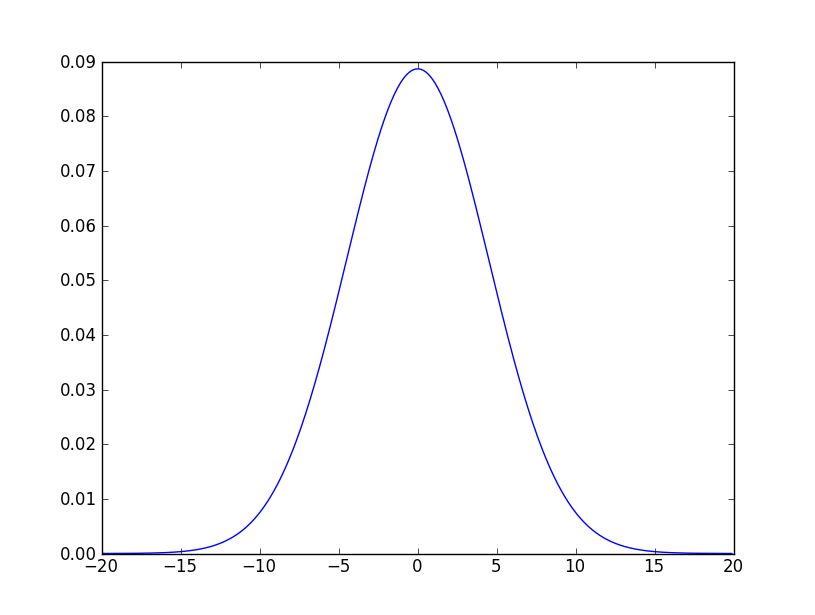
\includegraphics[width=1\linewidth]{img/cylinderGauss.png} \\ а)}
	\end{minipage}
	\hfill
	\begin{minipage}[h]{0.49\linewidth}
		\center{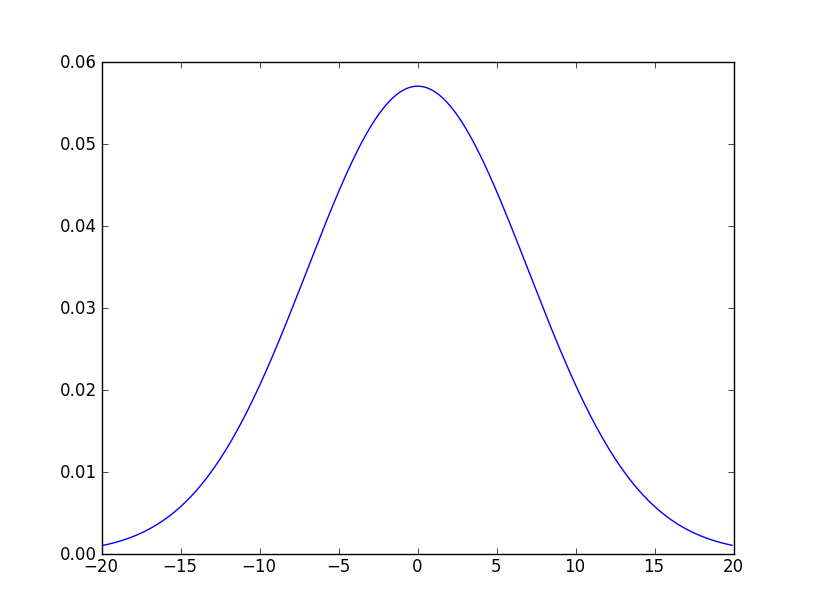
\includegraphics[width=1\linewidth]{img/planarGauss.png} \\ б)}
	\end{minipage}
	\caption{Распределение поля в волноводах: а) цилиндрический, б) планарный}
\end{figure}

Здесь видно, что эти поля не совпадают, следовательно при их соединении перейдёт не вся энергия, а только та часть, которая перекрывается обоими распределениями

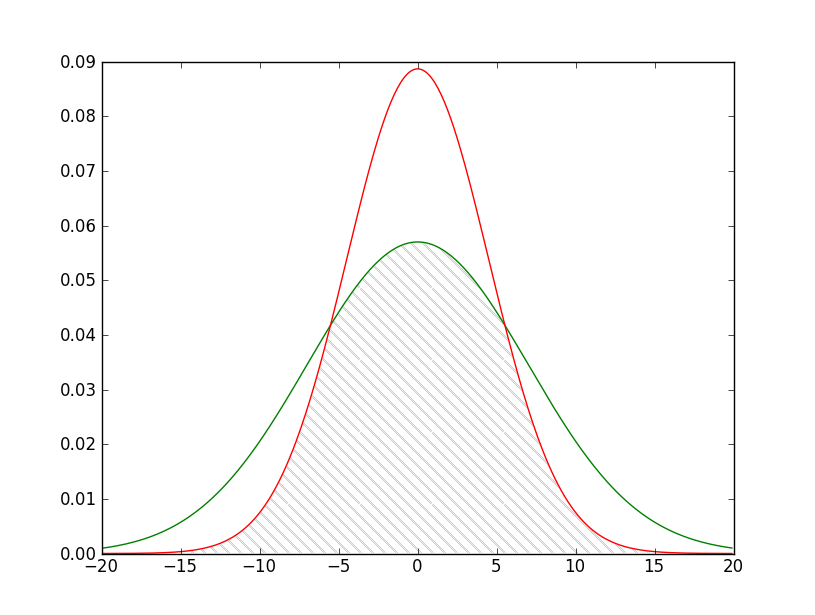
\includegraphics[width=0.5\textwidth]{img/intersection.png}

В случае, если волноводы совмещены не соосно, то площадь перекрытия уменьшается еще больше:

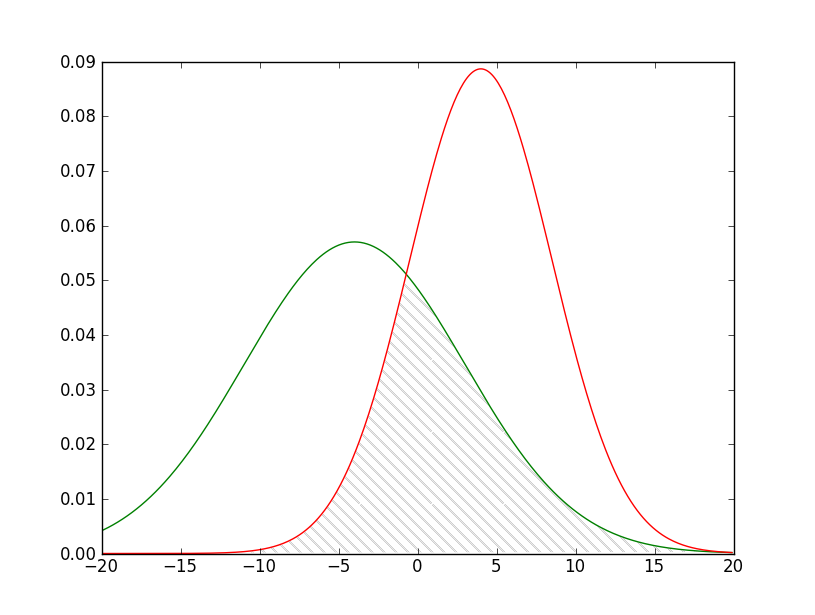
\includegraphics[width=0.5\textwidth]{img/intersection2.png}

Опишем эту зависимость теоретически.

Максимальная энергия поля в волноводе равна:
\begin{equation}
	W(x) = \int_{-\infty}^{\infty}E(x)dx = 1
\end{equation}

При контакте двух волноводов передается только та часть энергии, которая перекрывается обоими полями мод, остальная рассеивается, так как нарушает условия волноводного распространения. Таким образом, перешедшая энергия описывается так:

\begin{equation}
	\label{transition}
	W(x) = \int_{-\infty}^{\infty}min\bigl(E_1(x), E_2(x)\bigr)dx
\end{equation}
где $E_1$ и $E_2$ - распрелеление поля первого и второго волновода соответственно.

Эта величина максимальна и равна 1 при совпадении формы и центра каждого и уменьшается при увеличении расстояния между их центрами. Зафиксируем положение планарного волновода и будем перемещать центр цилиндрического, при этом будем вычислять значение интеграла (\ref{transition}). Воспользуемся для этого библиотекой scipy и языком программирования Python и получим график:
\begin{figure}[h!]
	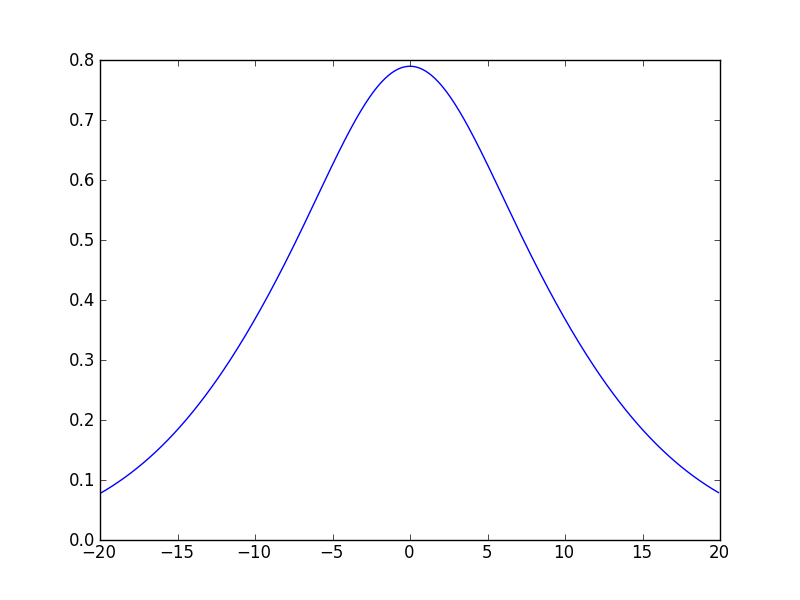
\includegraphics[width=0.5\textwidth]{img/transition.png}
	\caption{Зависимость к-та передачи от взаимного положения волноводов}
\end{figure}

\section{Поле волноводов в пространстве}

\begin{equation}
  \label{gauss2d}
  E(x,y)=\frac{1}{2\pi\sigma_1\sigma_2}\exp\left(-\frac{x^2}{2\sigma_1^2}-\frac{y^2}{2\sigma_2^2}\right)
\end{equation}


